\documentclass[letterpaper,journal]{IEEEtran}

\usepackage{amsmath}
\usepackage{graphicx}
\usepackage{cite}
\usepackage{url}
\usepackage{booktabs}
\usepackage{array}
\usepackage[caption=false,font=footnotesize]{subfig}
\usepackage{placeins}
\usepackage{float}
\raggedbottom

\newcolumntype{L}[1]{>{\raggedright\arraybackslash}p{#1}}

\begin{document}

\title{Non-Intrusive Load Monitoring with Harmonic Feature Fusion and Live On-the-Go Learning}

\author{Soheil Ayati and Marc Steffgen%
\thanks{Soheil Ayati and Marc Steffgen are with TH K\"oln (University of Applied Sciences), Faculty of Computer Science and Engineering Science, Campus Gummersbach, Germany.}%
\thanks{Modeling, Simulation and Automation of Electrical Energy Systems, Project Paper, submitted: July 2026.}%
}

\maketitle

\begin{abstract}
Non-intrusive load monitoring (NILM) estimates appliance-level consumption from one aggregate meter signal at the point of common coupling. This is attractive because it avoids sub-metering, but it becomes difficult when loads overlap, devices have similar active power, and behind-the-meter photovoltaic (PV) generation can mask or invert the net signal. This paper presents a complete laboratory NILM pipeline built around a Siemens SENTRON PAC4200 power meter. The system combines synthetic data with embedded ground truth, semi-synthetic mixes from real single-device recordings, harmonic feature fusion, and a live dashboard that can learn unknown devices during operation. The final Random Forest mix model reaches a held-out presence macro-F1 of 0.916 and a gated power mean absolute error of 2.9 W on 1920 measured-scenario windows. In live tests, the system detects switching events with millisecond timestamps, reports unexplained residual power instead of forcing wrong labels, and retrains after a guided unknown-device recording in 26 s. The results show that a low-frequency industrial meter can support useful NILM when steady-state, harmonic, phase, and transient information are treated as one coherent feature space.
\end{abstract}

\begin{IEEEkeywords}
Non-intrusive load monitoring, NILM, energy disaggregation, harmonic features, photovoltaic generation, PAC4200, Random Forest.
\end{IEEEkeywords}

\section{Introduction}

Detailed knowledge of appliance-level electricity use is valuable for energy feedback, laboratory monitoring, demand-side flexibility, and fault detection. Installing one meter per appliance provides this information directly, but it is intrusive, expensive, and difficult to maintain. NILM instead tries to recover appliance states and power contributions from a single aggregate measurement at the point of common coupling (PCC), an idea introduced by Hart through event-based load signatures in the active-reactive power plane \cite{hart1992nilm}.

This project addresses NILM in a small but realistic laboratory setting. The goal is not only to classify isolated appliance recordings, but to build an end-to-end system that can acquire data from a real power meter, train on reproducible labelled scenarios, infer which devices are active, estimate their wattage, and expose the result in a live interface. Two challenges motivate the design. First, behind-the-meter PV generation can create a signal eclipse: consumption and generation cancel in the aggregate signal, or net active power becomes negative \cite{wang2025dualnilm}. Second, many devices are not separable by active power alone. Low-power electronics, motors, lamps, and chargers may overlap in wattage while differing strongly in reactive power, power factor, current distortion, and switching dynamics. Prior NILM work has shown that feature fusion and harmonic content improve separability \cite{reddy2020featurefusion,papageorgiou2022odd}.

The contribution of this work is a complete NILM workflow tailored to the available hardware and project constraints: a synthetic-first data pipeline with exact per-sample ground truth, a real PAC4200 acquisition path, common HDF5 storage, physics-based aggregation including harmonic vector summation, compact physically interpretable features, tabular machine-learning models, and a live monitor with residual-based unknown-device teaching. The emphasis is practical transfer from a controlled project model to a running laboratory interface.

\section{Concept and System Design}

The central concept is source-agnostic processing. Synthetic scenarios and real meter recordings differ only in acquisition; after data are stored, preprocessing, feature extraction, training, inference, and live monitoring use the same code path, as shown in Fig.~\ref{fig:architecture}. Let $y(t)$ denote the aggregate meter signal and $p_i(t)$ the active power contribution of appliance $i$. NILM estimates
\begin{equation}
    \hat{\mathbf{p}}_{1:N}(w) = f_{\theta}(y_{t:t+w})
\end{equation}
over a fixed window $w$, together with binary presence labels. PV is treated as a normal signed contributor, with $p_i(t)<0$ during generation, so export and cancellation remain representable throughout the pipeline.

\begin{figure}[H]
\centering
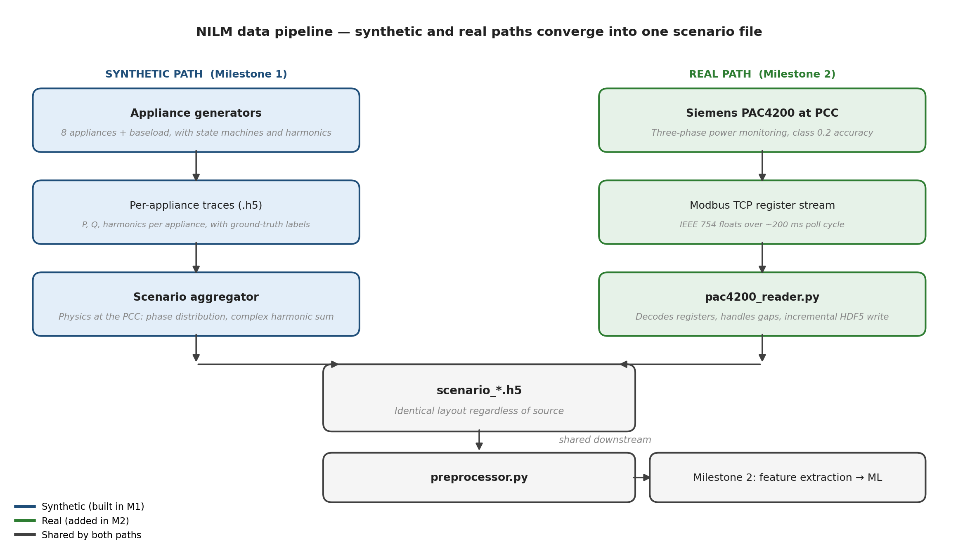
\includegraphics[width=\columnwidth]{figures/ms1_image1.png}
\caption{Milestone-1 architecture decision: synthetic appliance generation and real PAC4200 acquisition are different front ends that converge into the same scenario format. This made later ML and live processing source-agnostic instead of requiring separate code paths.}
\label{fig:architecture}
\end{figure}

\subsection{Why Synthetic and Measured Data Are Both Needed}

Synthetic data provide the supervision that real aggregate measurements lack. The project implements generators for fridge, resistive load, hair dryer, PC, washing machine, EV charging, PV, synchronous machine, and baseload. Each generator has a state model, time-of-day behaviour, active and reactive power, and current harmonics. Different seeds create different appliance instances. This allows controlled scenarios, including adversarial cases where PV masks load.

Real data are still necessary because a purely synthetic model may learn idealised signatures. The PAC4200 reader records isolated devices in the laboratory. A measured-scenario mixer then loops these real single-device recordings with random on/off schedules and feeds them through the same aggregation format as the synthetic path. This yields aggregate measured scenarios with exact ground truth while preserving real device signatures.

Fig.~\ref{fig:ms1_signals} shows how the early synthetic work later shaped the ML design. The PV trace forced signed active power and negative aggregate values into the data model from the beginning. The 24 h aggregate scenario then made the actual NILM task explicit: the model only observes the PCC-level signal, while the per-appliance breakdown is available only as training ground truth.

\begin{figure}[H]
\centering
\subfloat[PV: signed generation.]{
    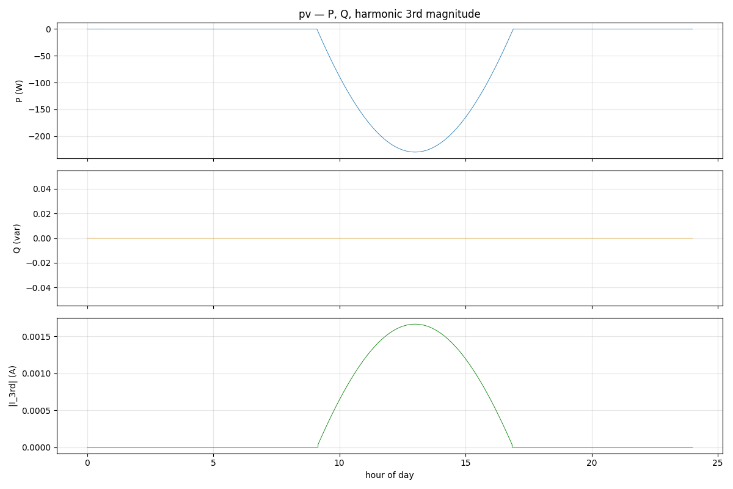
\includegraphics[width=0.95\columnwidth]{figures/ms1_image4.png}
}\\
\subfloat[24 h PCC aggregate and hidden ground truth.]{
    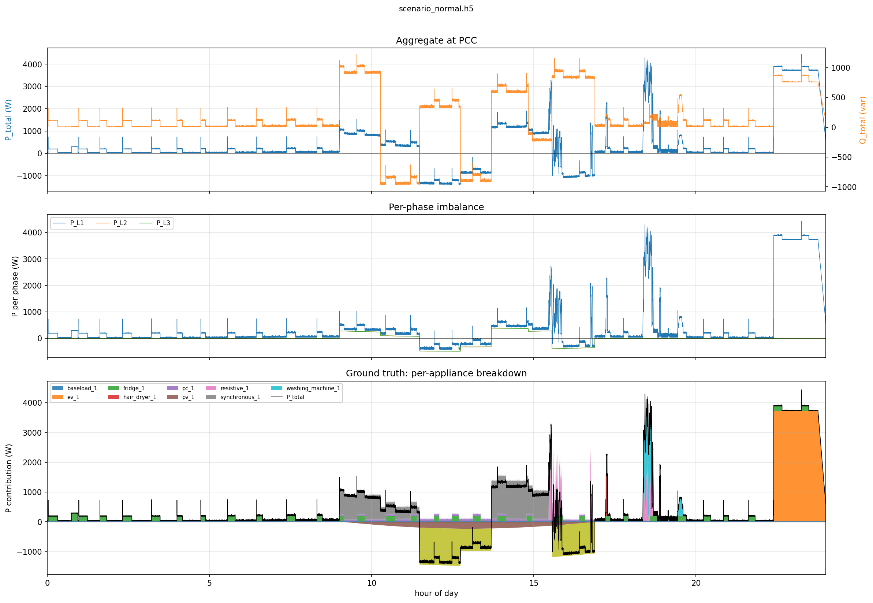
\includegraphics[width=0.95\columnwidth]{figures/ms1_image5.png}
}
\caption{Milestone-1 findings that carried into the final system: signed PV generation, aggregate-only observation at the PCC, and per-appliance ground truth for supervised learning.}
\label{fig:ms1_signals}
\end{figure}

\subsection{Why Harmonics Matter}

The PAC4200 cannot stream raw waveforms over Modbus TCP; it exposes processed RMS, power, power factor, and harmonic quantities. A full polling cycle is realistically about 200 ms, so the system operates at 5 Hz. This excludes sub-cycle waveform methods, but it still captures steady-state signatures, second-scale transients, and per-order current harmonics.

Harmonics are important because active power alone is ambiguous. In the project's real fingerprint measurements, a 6.7 W LED lamp and a 10 W USB charger are close in active power, while their current THD differs strongly. Likewise, a fluorescent tube and a small motor can both have poor power factor for different physical reasons. The implemented feature space therefore combines active power, reactive power, apparent power, power factor, THD, low-order harmonics, phase localisation, and switching-step information.

\section{Implementation}

\subsection{Storage, Aggregation, and Preprocessing}

All main artifacts use HDF5. Files contain timestamps, measurements, metadata, and, where available, ground truth. Timestamps are stored as UTC microseconds, measurement channels as \texttt{float32}, and datasets are LZF-compressed. The format is shared by synthetic single-device traces, aggregate scenarios, PAC4200 recordings, and preprocessed outputs.

The aggregator mimics what the meter observes at the PCC. Single-phase devices contribute to one phase; three-phase PV and synchronous-machine models are distributed equally across phases. Harmonics are not summed by magnitude. For each phase $\phi$ and order $n$, appliance harmonic contributions are added as complex vectors,
\begin{equation}
    I_{n,\phi}^{\mathrm{agg}}(t) =
    \sum_i a_{i,\phi} I_{i,n}(t)e^{j\varphi_{i,n}(t)} ,
\end{equation}
and stored as magnitude and phase. This is necessary because equal harmonic orders can cancel or reinforce depending on phase angle. The preprocessor then validates files, imputes gaps up to five samples (1 s at 5 Hz), clips physically impossible outliers, and writes cleaned channels plus derived features without modifying raw measurements.

\subsection{PAC4200 Reader and Live Acquisition}

The real acquisition tool maintains one persistent Modbus TCP connection to the Siemens SENTRON PAC4200. It polls the verified core map for voltage, current, active/reactive/apparent power, power factor, frequency, and totals. Harmonic magnitudes are read via Modbus function code 0x14 file records rather than a normal register block; on the tested device, current harmonic file 113 on L1 was verified against a real load. The meter provides harmonic magnitudes but not harmonic phases, so real recordings mark phase data as unavailable and models intended for deployment avoid synthetic-only phase features. Siemens documentation defines the available metering quantities and communication basis \cite{siemens2023pac4200}.

The second milestone converted real single-device recordings into labelled measured scenarios. This was the decisive bridge from clean synthetic supervision to laboratory data: real appliance signatures were preserved, but the aggregate still carried exact per-device ground truth. Fig.~\ref{fig:ms2_measured} shows such a measured scenario and the corresponding presence evaluation.

\begin{figure}[H]
\centering
\subfloat[Measured mix with exact ground truth.]{
    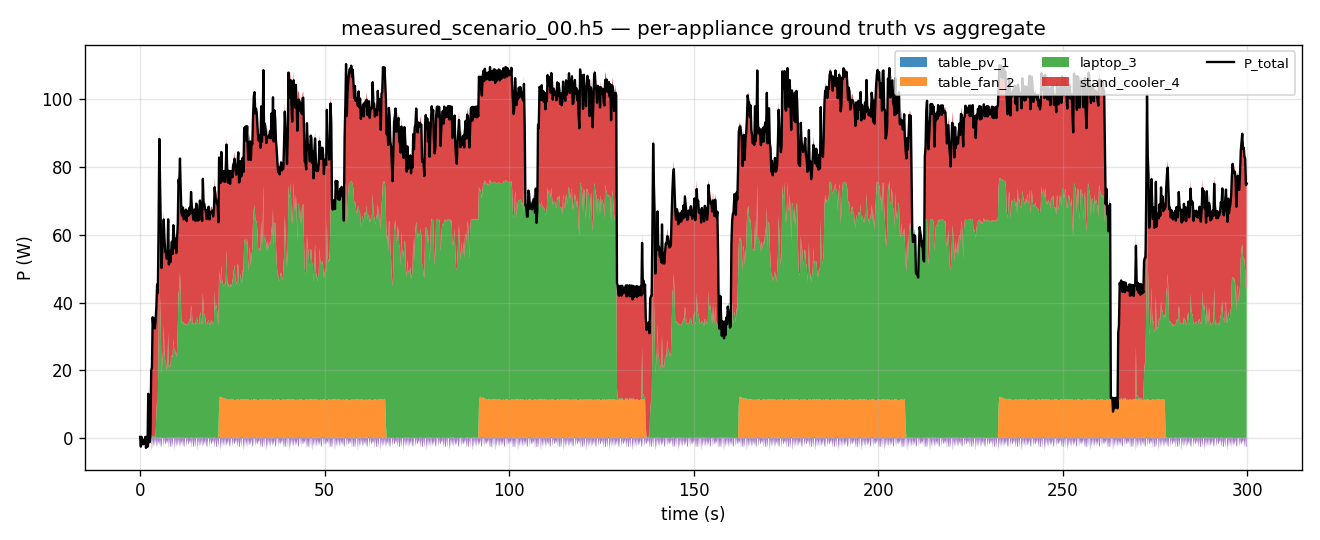
\includegraphics[width=\columnwidth]{figures/ms2_image2.png}
}\\
\subfloat[Presence prediction and ground truth.]{
    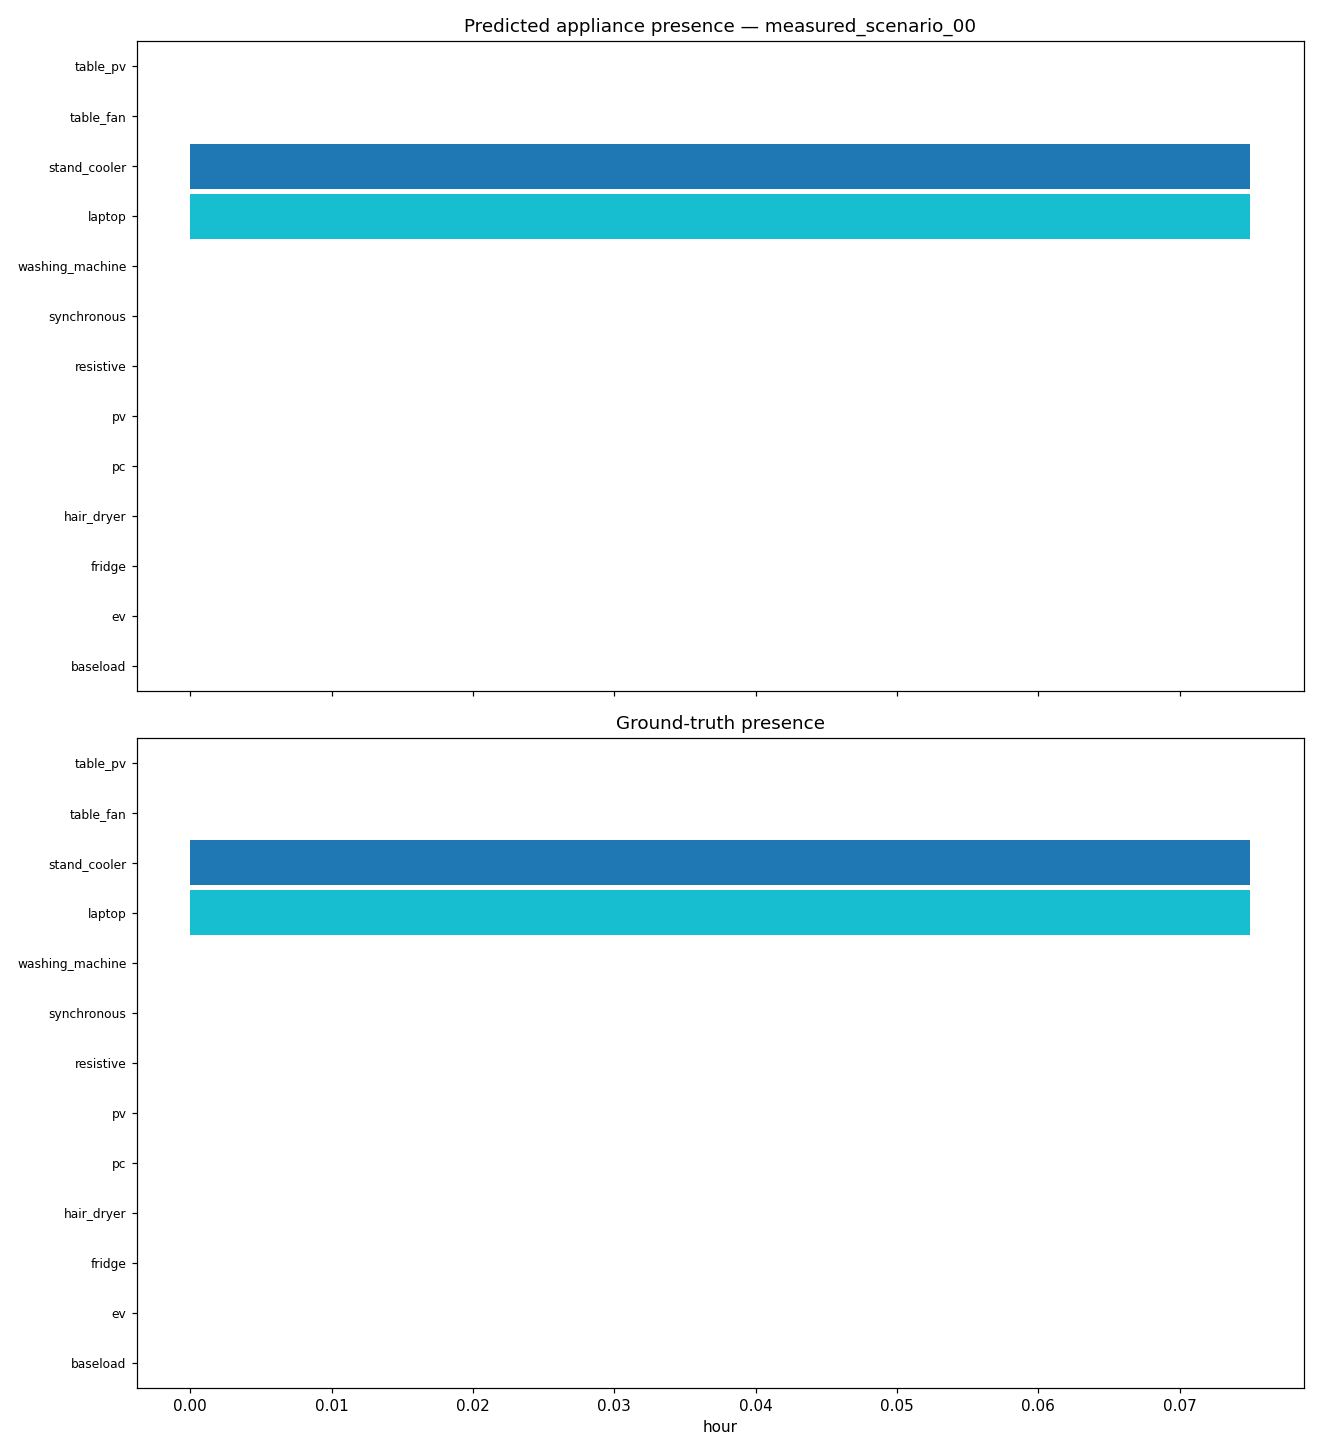
\includegraphics[width=0.7\columnwidth]{figures/ms2_image3.png}
}
\caption{Milestone-2 bridge from infrastructure to supervised NILM on measured laboratory signatures. Small or near-zero devices reveal threshold limits that later motivated residual handling.}
\label{fig:ms2_measured}
\end{figure}

\subsection{Models and Features}

The implemented ML pipeline supports four tasks: \emph{identify} maps an isolated-device window to one label; \emph{disaggregate} estimates watts per appliance; \emph{presence} predicts multi-label on/off states; and \emph{mix} combines presence and gated power estimation in one deployable bundle. Random Forest is the default model because the data regime is small, features are tabular and interpretable, and retraining must finish quickly enough for live use. LightGBM provides a second tree-based baseline, while a scikit-learn MLP serves as a simple neural path. More specialised sequence models such as seq2point or neural NILM remain natural follow-up work \cite{zhang2018seq2point,kelly2015neural}.

Table~\ref{tab:features} summarises the main feature groups. The current mix model uses 17 aggregate features over 10 s windows. The last three event features were added for the live system: the largest settled active-power step, the reactive step at the same instant, and the number of steps in the window. These inject Hart-style transient information into a window model.

\begin{table}[H]
\caption{Feature groups used by the NILM pipeline.}
\label{tab:features}
\centering
\renewcommand{\arraystretch}{1.05}
\begin{tabular}{L{0.24\columnwidth}L{0.65\columnwidth}}
\toprule
\textbf{Group} & \textbf{Examples and purpose} \\
\midrule
Steady state & $P$, $Q$, $S$, power factor, $Q/P$, and power statistics; separates load magnitude and type. \\
Phase & Per-phase active power; localises single-phase loads and balanced devices. \\
Harmonic & THD, 3rd/5th/7th order, spectral centroid, harmonic energy; captures nonlinear and motor signatures. \\
Transient & Settled $P/Q$ step and step count; adds switching information to window features. \\
Context & Hour of day for synthetic daily scenarios. \\
\bottomrule
\end{tabular}
\end{table}

\FloatBarrier

\subsection{Live NILM and Training on the Go}

The live monitor evaluates the trailing model window every few seconds and publishes device state, watts, confidence, model provenance, and explained-power fraction. Presence probabilities are median-smoothed and passed through hysteresis to avoid flicker. In parallel, an edge detector compares settled medians before and after a change in $P$ and $Q$. Matched edges claim or release device states directly, which improves timing and prevents a steady-state model from explaining a new lamp as a drift of an already active boiler.

Unexplained residual power is an explicit output of the system. If the measured aggregate is not sufficiently explained for at least eight seconds, the dashboard prompts the user to teach the unknown device. The final protocol records a clean isolated device signature: all devices off, short baseline, only the new device on, and off tail. The system then rebuilds measured scenarios, retrains the mix and identify bundles, and hot-reloads them without restarting the session.

The three final live tests in Fig.~\ref{fig:live_screens} illustrate the implementation from the operator's perspective. The first screen is a low-power case: the standing fan is edge-confirmed, a small table fan is detected with lower wattage, and the residual remains visible instead of being hidden. The second screen shows an expanded vocabulary after adding devices such as a laptop; it also logs an unrecognised edge when no known device signature matches. The third screen is the high-load case: several devices are separated simultaneously while the dashboard reports the explained-power fraction.

\begin{figure}[H]
\centering
\subfloat[Low-power split with residual.]{
    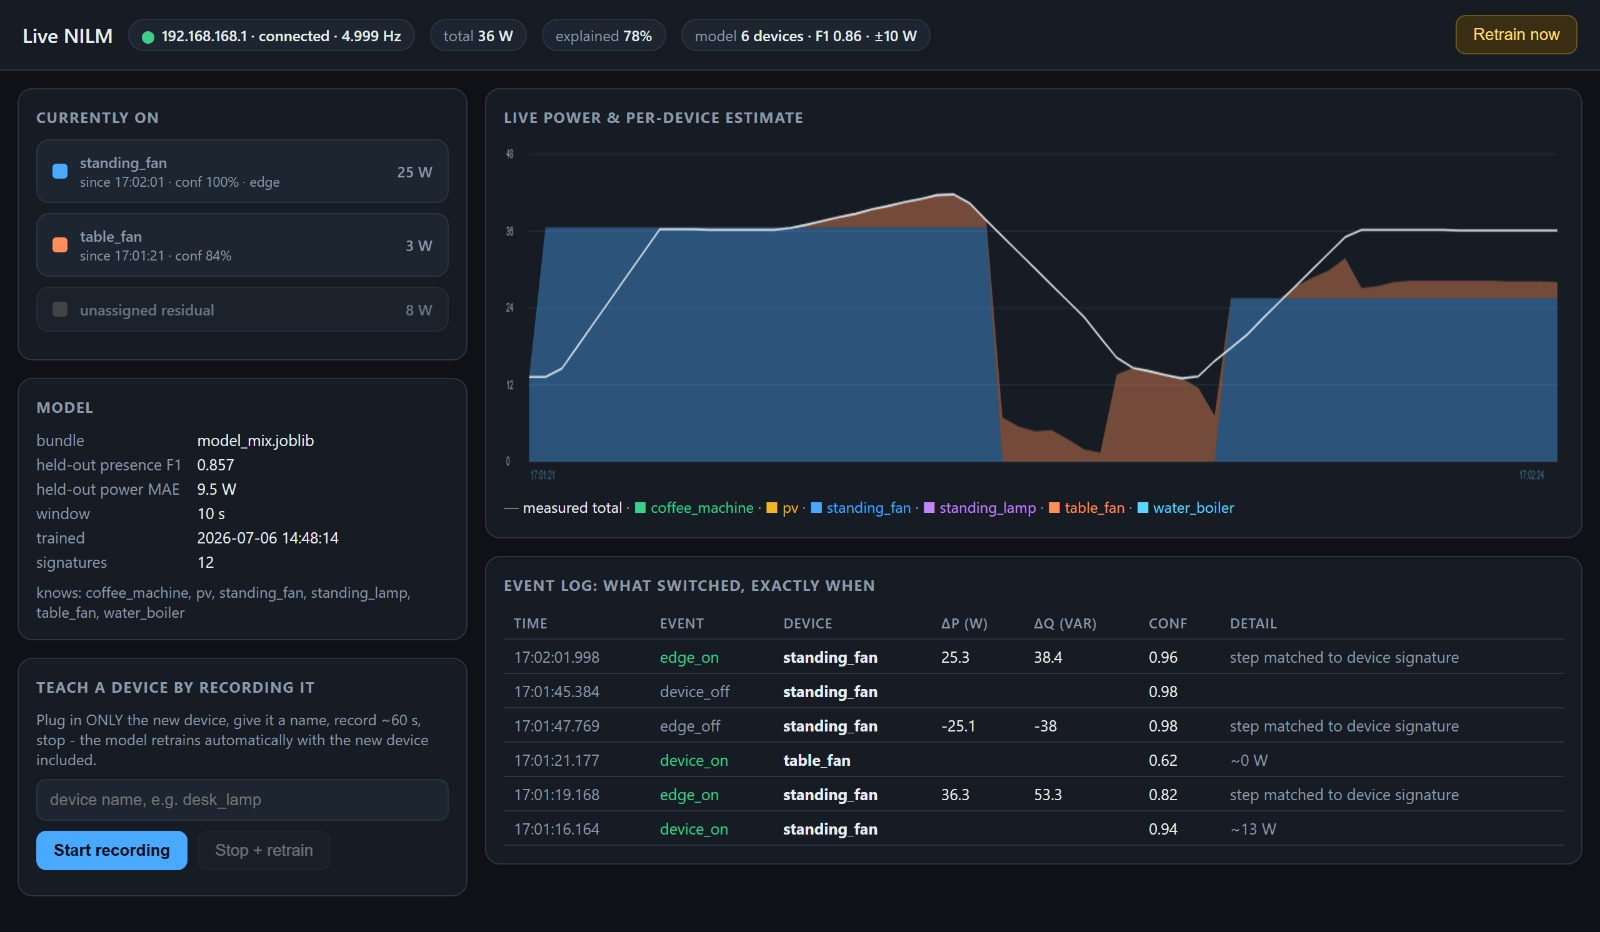
\includegraphics[width=0.82\columnwidth]{figures/live_test1.jpeg}
}\\
\subfloat[Expanded vocabulary and unrecognised edge.]{
    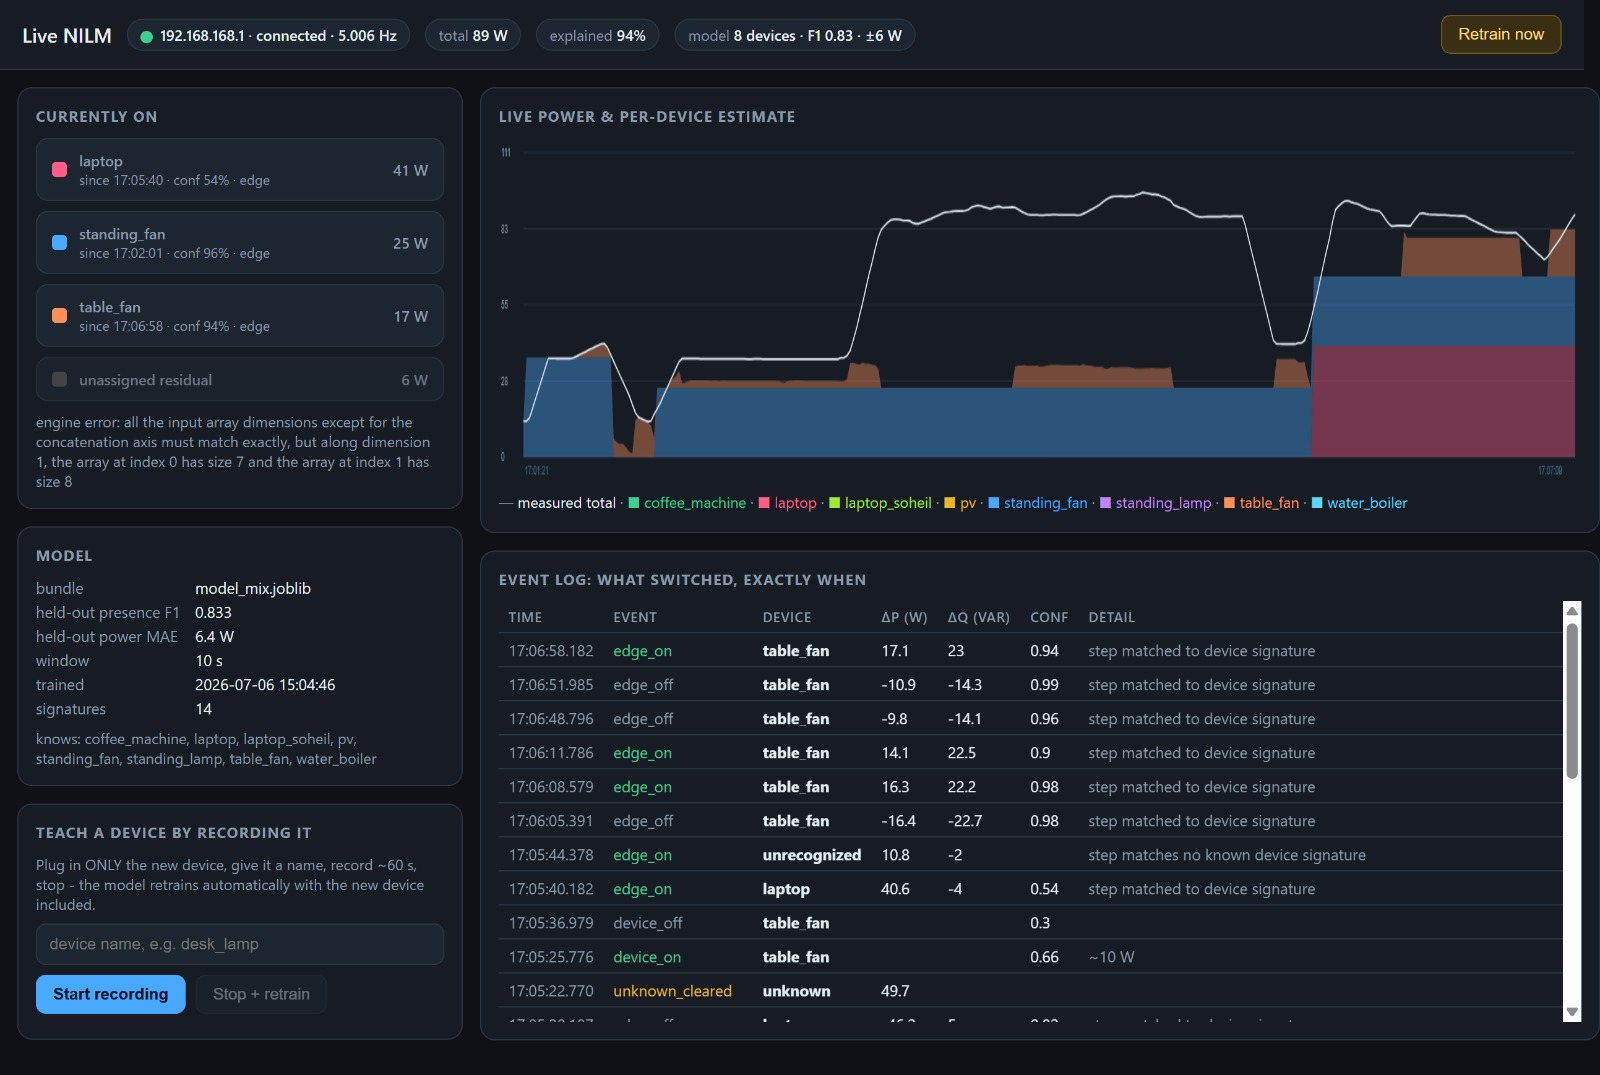
\includegraphics[width=0.82\columnwidth]{figures/live_test2.jpeg}
}\\
\subfloat[High-load multi-device split.]{
    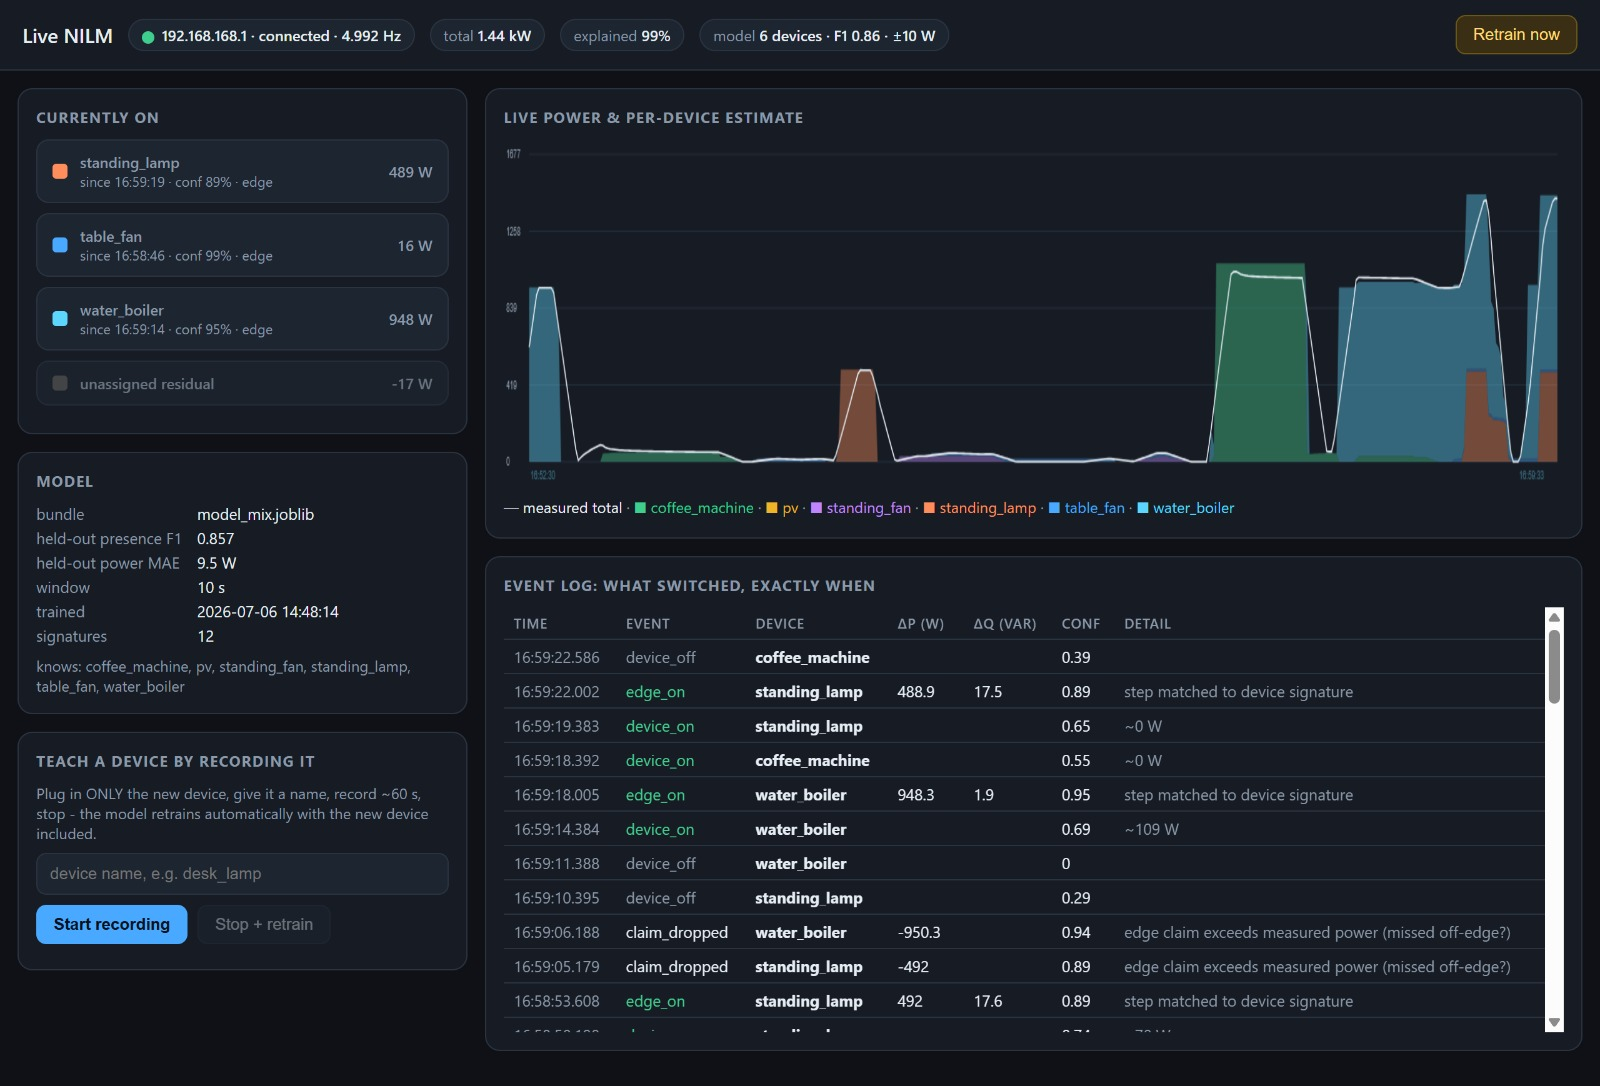
\includegraphics[width=0.82\columnwidth]{figures/live_test3.jpeg}
}
\caption{Milestone-3 live dashboard snapshots. The interface combines current device states, stacked per-device estimates, measured aggregate power, model metrics, residual power, and an event log with matched switching edges.}
\label{fig:live_screens}
\end{figure}

\section{Results}

The current measured-data mix model is trained on 1920 windows from measured scenarios with a 10 s window and a 5 W on-threshold. Its vocabulary contains coffee machine, laptop, PV, standing fan, standing lamp, table fan, and water boiler. Held-out presence macro-F1 is 0.916 and gated power MAE is 2.9 W. The identify bundle, trained on 171 active real-device windows with common plus harmonic features, reaches held-out macro-F1 0.955 and accuracy 0.953; this result uses a stratified row split because there is currently only one recording session per family, so it should be interpreted as an optimistic within-session estimate.

The live validation demonstrates the system-level behaviour. The teach loop detects an unknown load after 8 s, retrains in 26 s, and subsequently recognises the taught device with 0.95 confidence while explaining 97.9\% of the measured power. In the high-load dashboard snapshot in Fig.~\ref{fig:live_screens}(c), about 1.44 kW is split into water boiler, standing lamp, and table fan with 99\% explained power.

The key qualitative result is that the system does not force every watt into a known appliance. Small unexplained loads remain visible as residuals; unmatched switching steps are logged as unrecognised events; and the user can turn such residuals into training data. This is important for NILM deployment, where a wrong confident answer is often less useful than an explicit ``unknown'' state.

\section{Discussion}

The project confirms that a 5 Hz industrial meter can support a useful NILM system when the algorithm is designed around the meter's actual information content. The strongest design decision is the common pipeline for synthetic, measured, offline, and live data. Synthetic scenarios provide complete supervision and difficult PV cases; measured single-device recordings bring real hardware signatures; the measured-scenario mixer connects both without creating a separate ML path.

Several limitations remain. Real PV disaggregation is not validated because the available PV recording contains almost no actual generation; the synthetic PV path demonstrates sign handling and signal-eclipse logic, but not transfer to a producing inverter. The two small fans overlap strongly in $P/Q$ space and need more variant recordings. Harmonic phases are synthetic-only because the PAC4200 does not expose them over Modbus. The measured mixes are semi-synthetic, so real simultaneous-device interactions are only partially tested by held-out multi-device recordings. Finally, longer appliances such as washing machines are better suited to CNN/LSTM-style temporal models than to independent 10 s windows.

Within these constraints, the result is a complete proof of concept rather than only a classifier. It records, trains, infers, explains confidence, logs events, detects the unknown, and updates itself. This moves NILM from an offline score toward an operator-facing system that can be used and improved in a real laboratory setting.

\section{Conclusion}

This paper presented a PV-aware NILM pipeline that combines signed aggregate power, harmonic feature fusion, synthetic ground truth, measured laboratory recordings, and live training on the go. The system reaches 0.916 held-out presence macro-F1 and 2.9 W gated MAE on measured scenarios, while the live interface demonstrates event-level timing, residual monitoring, and fast retraining for unknown devices. Future work should record real PV generation, expand repeated recording sessions for leakage-free grouped evaluation, and replace the simple MLP path with sequence models that can exploit multi-minute appliance cycles.

\hfill \break


\FloatBarrier

\bibliographystyle{IEEEtran}
\bibliography{references}

\end{document}
